\documentclass{article} % For LaTeX2e
\usepackage{nips2016,times}
\usepackage{hyperref}
\usepackage{url}
\usepackage{graphicx}
%\documentstyle[nips14submit_09,times,art10]{article} % For LaTeX 2.09


\title{Fast Neighborhood Graph Converge based on Orientation Sensitive Hashing}


\author{
David S.~Hippocampus\thanks{ Use footnote for providing further information
about author (webpage, alternative address)---\emph{not} for acknowledging
funding agencies.} \\
Department of Computer Science\\
Cranberry-Lemon University\\
Pittsburgh, PA 15213 \\
\texttt{hippo@cs.cranberry-lemon.edu} \\
\And
Coauthor \\
Affiliation \\
Address \\
\texttt{email} \\
\AND
Coauthor \\
Affiliation \\
Address \\
\texttt{email} \\
\And
Coauthor \\
Affiliation \\
Address \\
\texttt{email} \\
\And
Coauthor \\
Affiliation \\
Address \\
\texttt{email} \\
(if needed)\\
}

% The \author macro works with any number of authors. There are two commands
% used to separate the names and addresses of multiple authors: \And and \AND.
%
% Using \And between authors leaves it to \LaTeX{} to determine where to break
% the lines. Using \AND forces a linebreak at that point. So, if \LaTeX{}
% puts 3 of 4 authors names on the first line, and the last on the second
% line, try using \AND instead of \And before the third author name.

\newcommand{\fix}{\marginpar{FIX}}
\newcommand{\new}{\marginpar{NEW}}

%\nipsfinalcopy % Uncomment for camera-ready version

\begin{document}


\maketitle

\begin{abstract}
Converge on neighborhood graph tends to encounter a lot of disk page accesses. We present a technique called OSH (Orientation Sensitive Hashing) to prevent from wasting unnecessary disk page accesses. Inspired by LSH, we find that during the expansion, neighbors that are closer to the query are more like to provide valid converge path. However, most methods do not pay attention on filter out further neighbors which we consider as false positives (or unnecessary points) during the expansion.

OSH can register the orientation of all neighbors of a node. During the ANN search, the orientation of the query w.r.t the current node can also be figured out quickly. We then sort all the orientation bit string and firstly choose the one with the most same orientation to expand. 
\end{abstract}

\section{Our Motivation}
\textbf{We see how many places we can apply our OSH techniques.}

\section{Introduction}\label{sec:intro}
\subsection{Search algorithms on NNG}\label{ssec:search_algorithm}
There has been a development over the search algorithms on NNG (or $k$-NNG).

A naive algorithm is the downhill search algorithm, as shown in Fig. \ref{fig:search_downhill}.
\begin{figure}
	\centering
	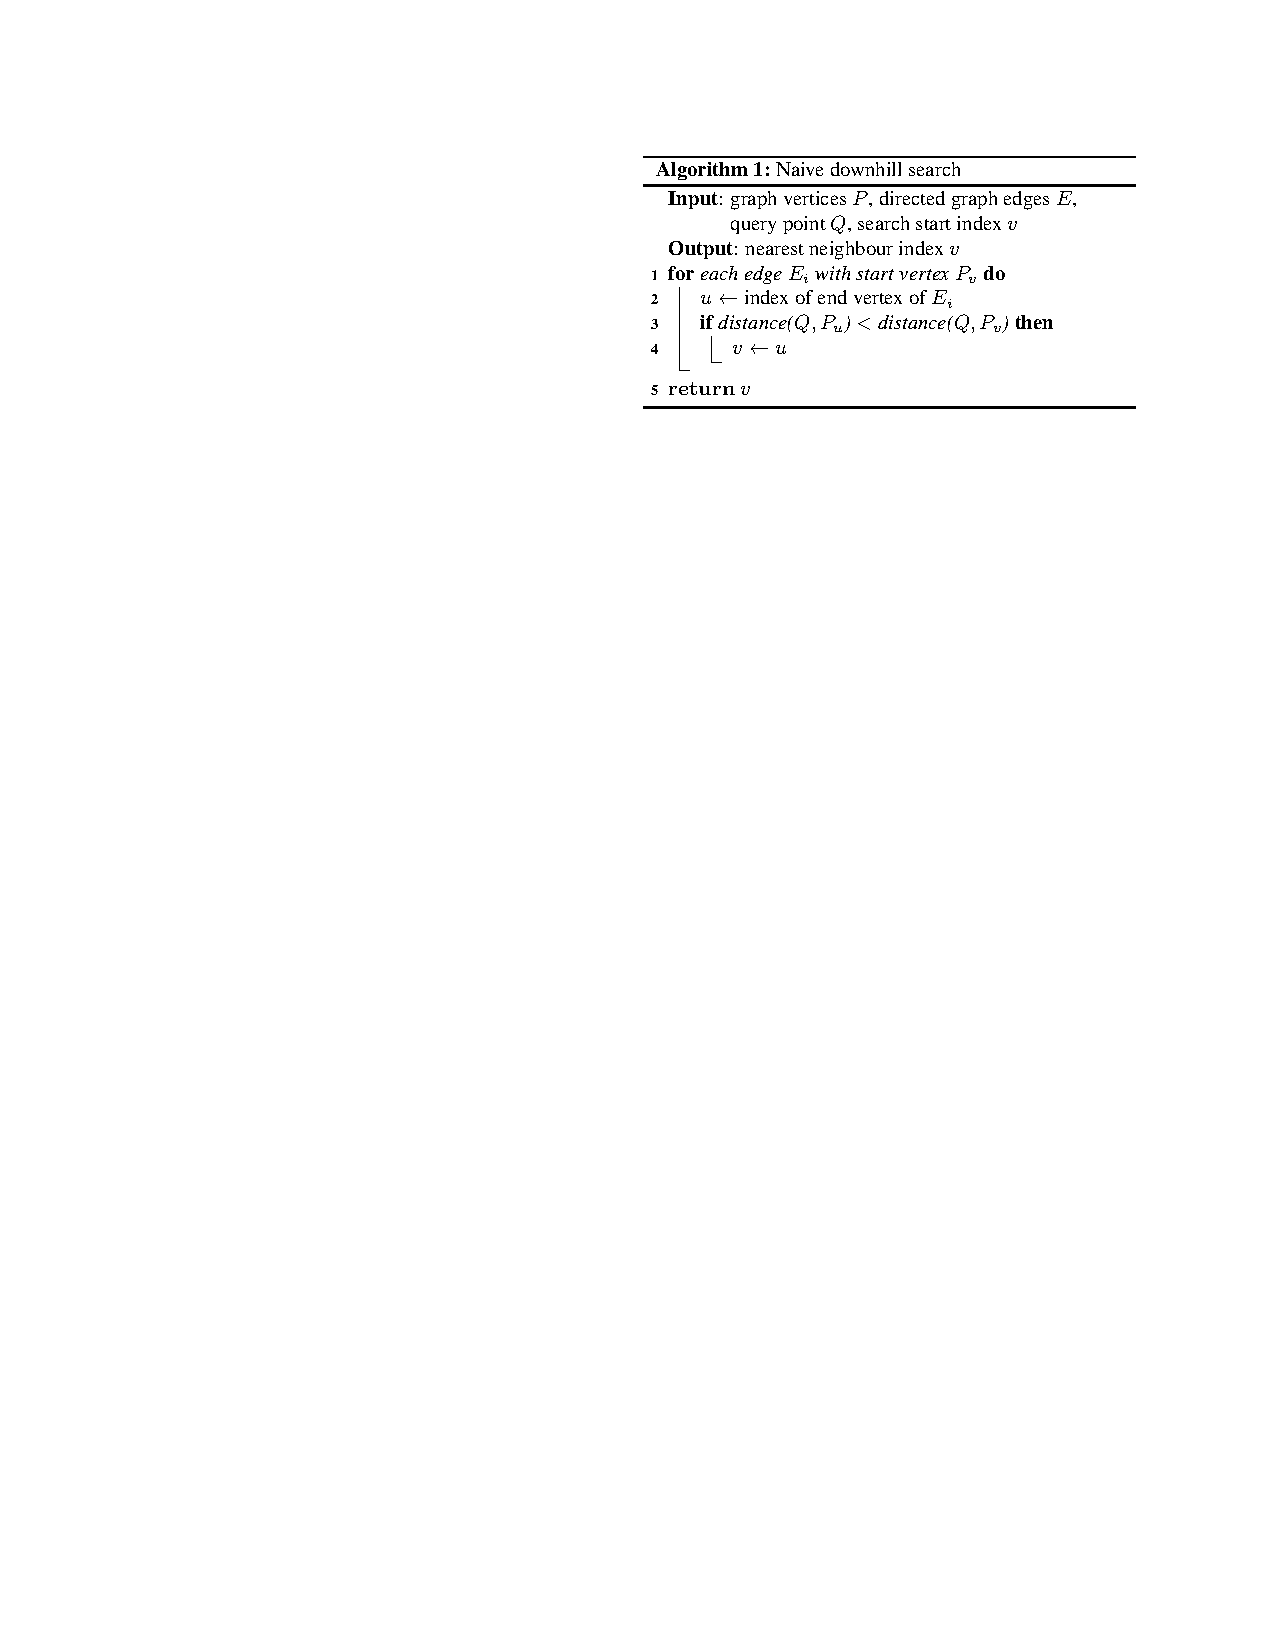
\includegraphics[width=0.45\textwidth]{search_downhill.pdf} \\
	\caption{Downhill search algorithm}\label{fig:search_downhill}
\end{figure}


In \cite{KianaFkNNG2011IJCAI}, the authors uses a ``best-first" strategy to search NNs: start from a random point $Y_0$, expand to the best neighbor among its $E$ neighbors, until it reaches a point who is better than any of its neighbor. Collect all encountered $E$ neighbors, find best $K$ ones as the $K$-NN search result. \textbf{The efficiency is very plain, the speedup around 3-16 on a 17k SIFT datasets with $K=30$}. 
\begin{figure}
	\centering
	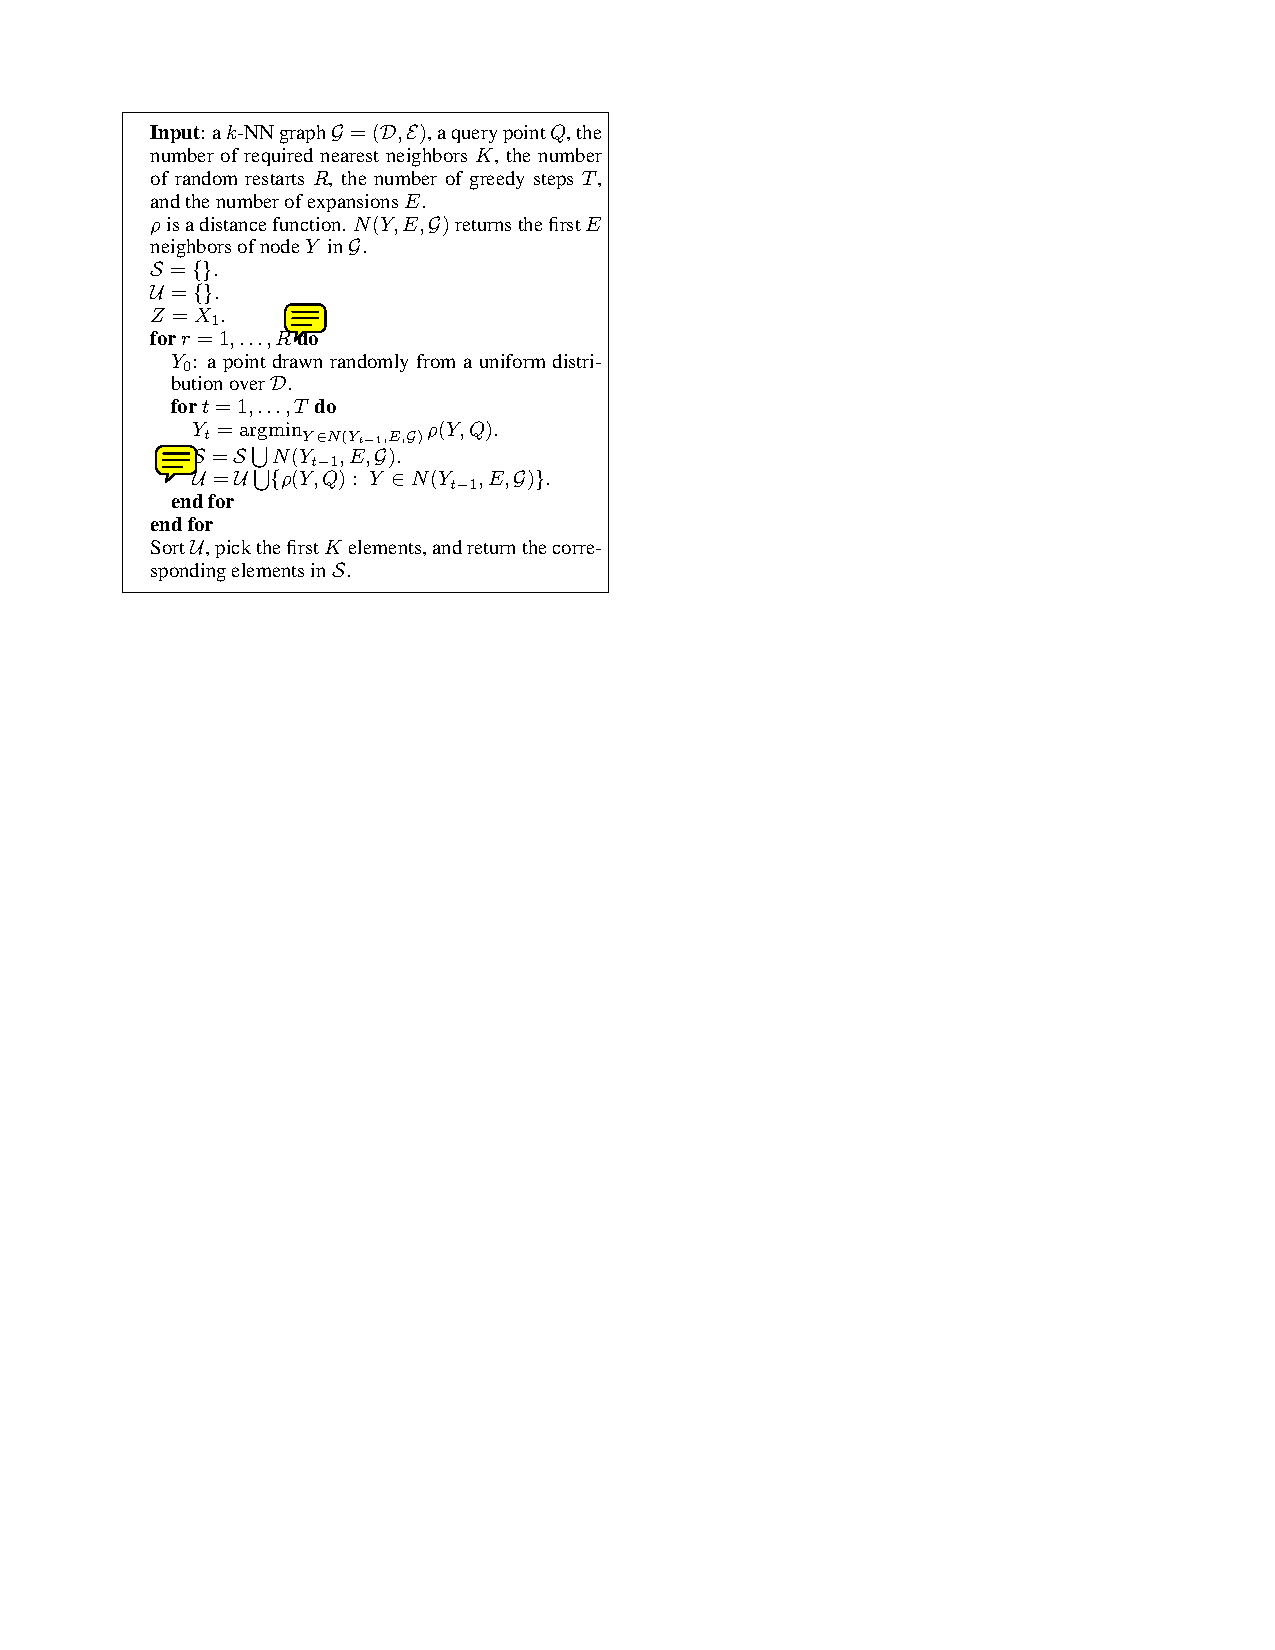
\includegraphics[width=0.45\textwidth]{search_FkNNG.pdf}
	\caption{NN Search in FkNNG}\label{fig:search_fknng}
\end{figure}


FANNG~\cite{HarwoodD2016FANNG} proposes a backtrack search algorithm, which is some kind of confused, I cannot understand yet. It seems like a greedy strategy, because it will move to a nearer node once found a nearer one. What confuses me is the priority query stores edges instead of nodes. Now I understand, all the edges are sorted according to the distance between the start point and the query.

$>$ Our technique can help to provide a sorted edge list in the ascending order of the distance to the query, in order to speedup the convergence, as shown in Fig. \ref{fig:search_backtrack}. 
\begin{figure}
	\centering
	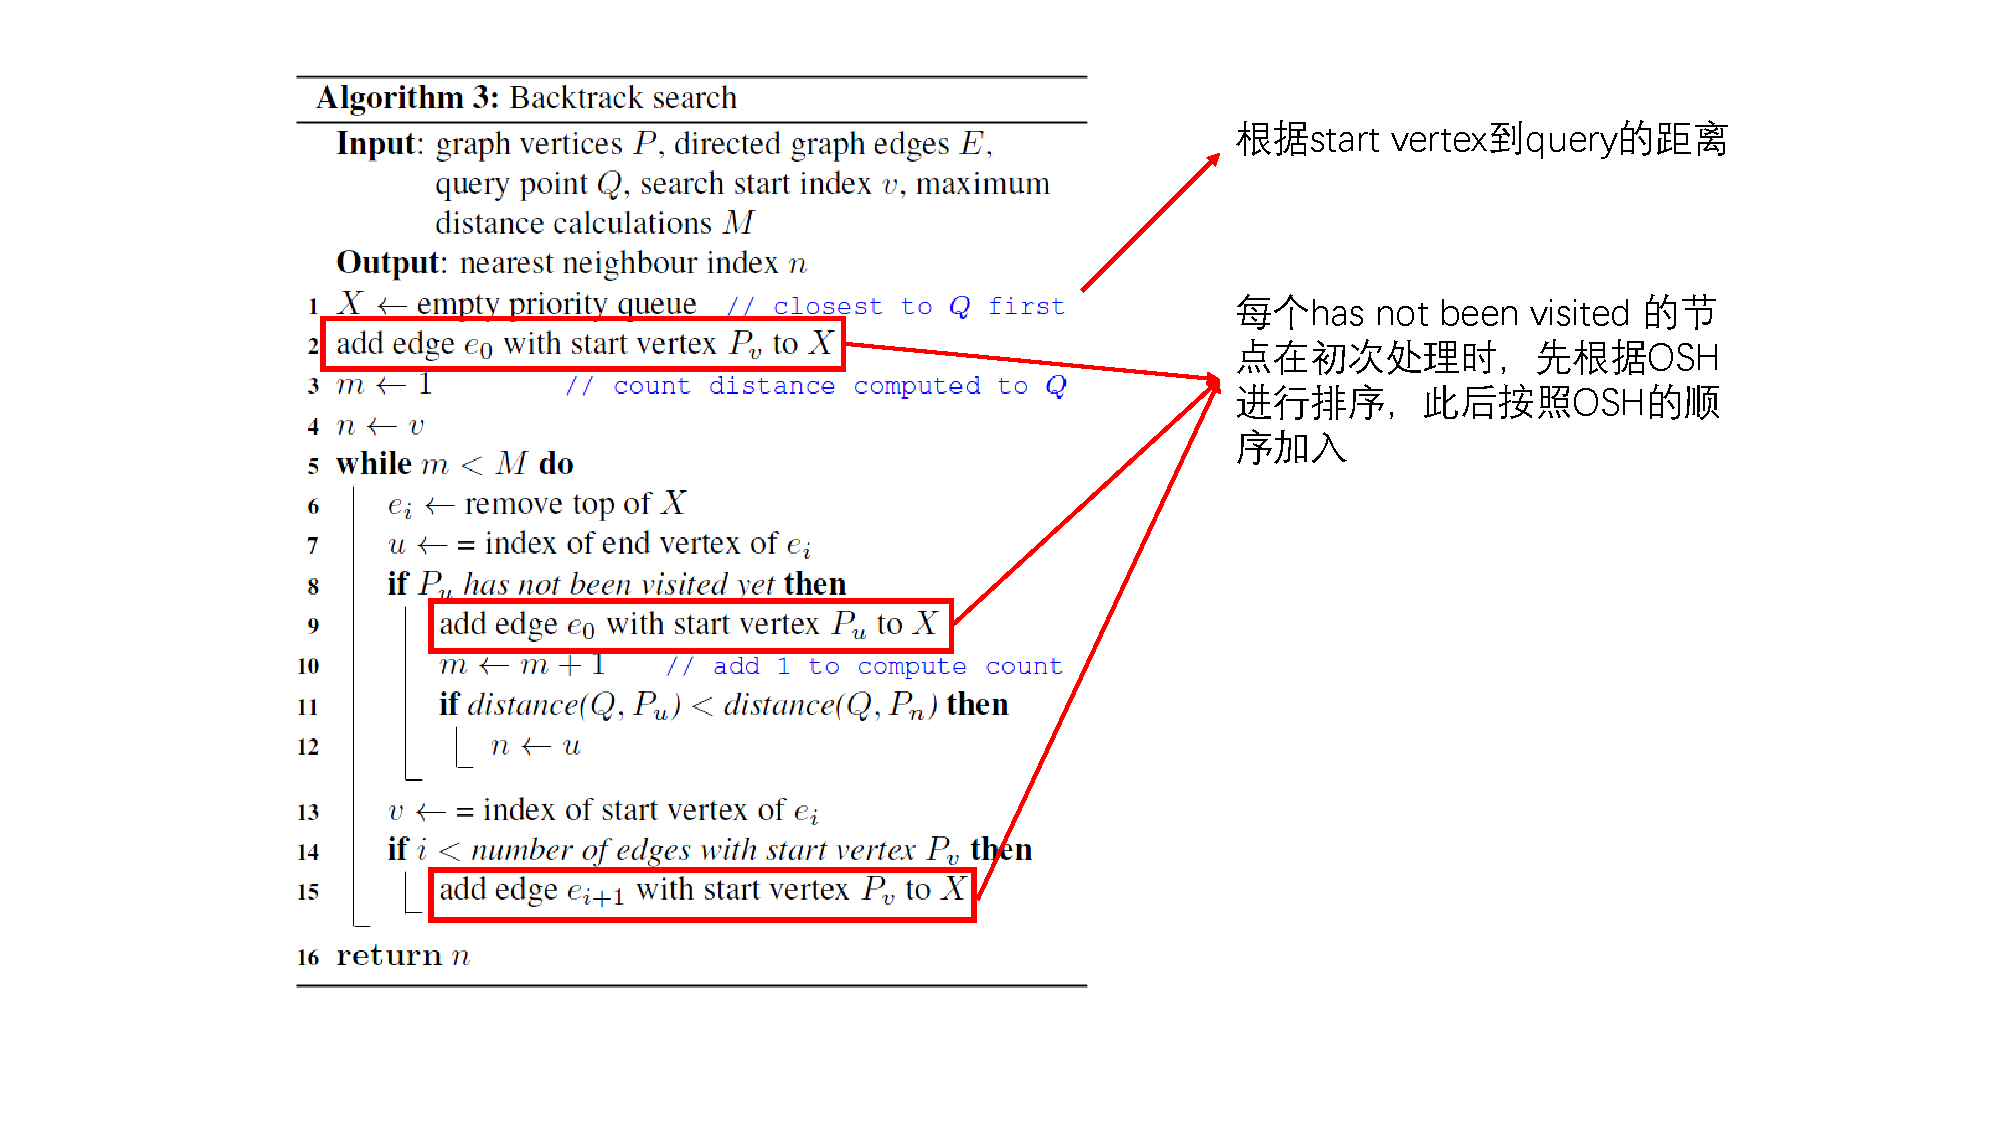
\includegraphics[width=0.8\textwidth]{search_backtrack.pdf}
	\caption{NN Search in FkNNG}\label{fig:search_backtrack}
\end{figure}


NNGPQ~\cite{WangJDNNGPQ2013} uses a combination of kNNG and a bridge NNG. During the search, it uses a priority queue $Q$ of data points. Each time pop out a best one, expand all its neighbors, push them into the $Q$ and also update the ANN result.

$>$ It is concerned that there is a case which we do not take into account. If we only expand neighbors that are closer than the current point $O$, when $O$ is quite near to the query, a neighbor of $O$ which is even further than $O$ can be a true NN. For this case, we say that for all neighbors that are closer to $O$ we consider, 

\section{Sketch of orientation sensitive hashing}\label{osh}

Orientation sensitive, as the term suggests, means that we want to seize the orientation similarity between data points.

\subsection{Definition of orientation}
Suppose there is a reference point $o \in R^d$, given two data points $p$ and $q$ we define the orientation of $p$ w.r.t $q$ as whether $p$ and $q$ located at the same side of the hyperplane $H_{qo}^{\bot}$, i.e.,
\begin{equation}
orient_q(p)=sign(op\cdot oq)
\end{equation}

\begin{figure}
	\centering
	% Requires \usepackage{graphicx}
	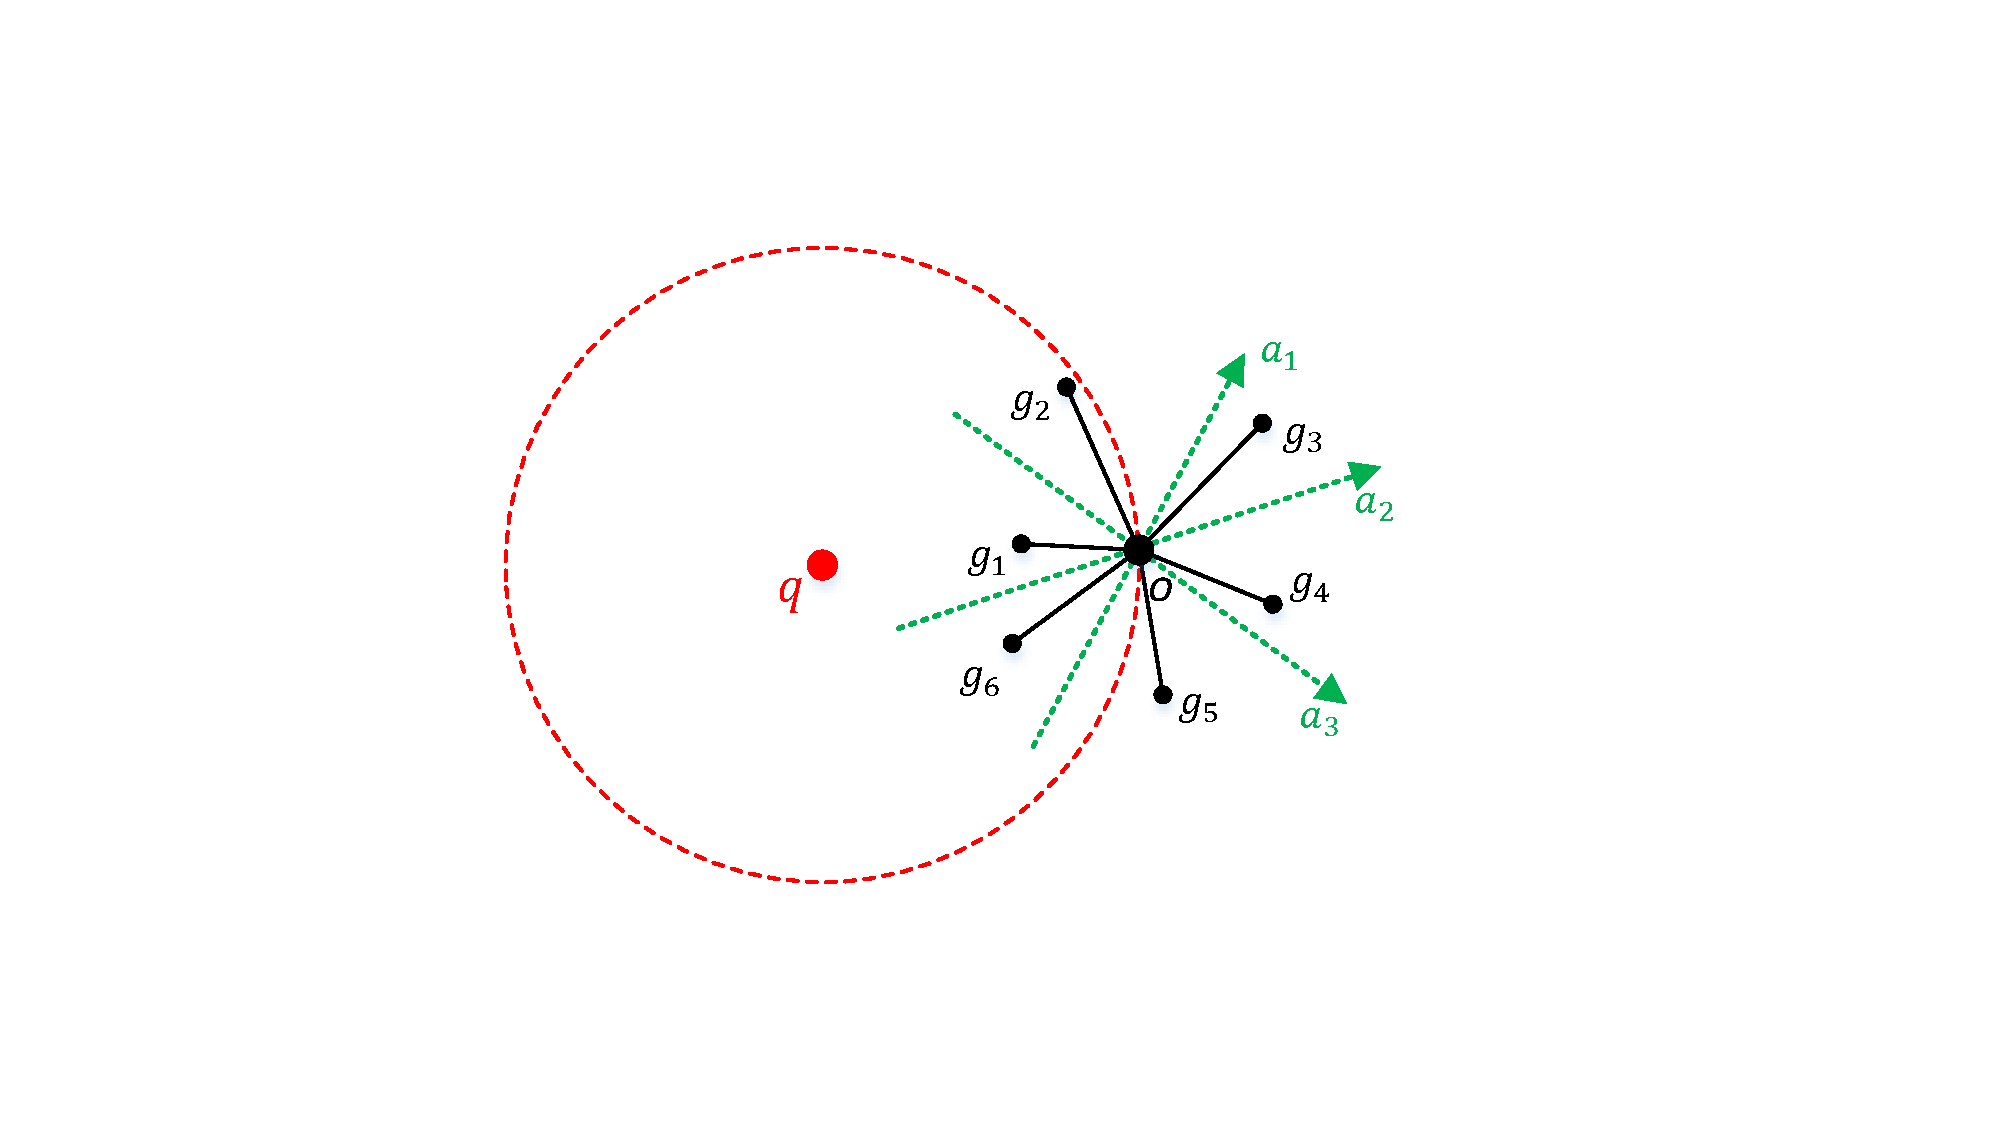
\includegraphics[width=0.45\textwidth]{OSH.pdf}\\
	\caption{Sample of orientation hashing}\label{fig:nncompare}
\end{figure}


\section{Related Works}






\subsection*{Acknowledgments}

Use unnumbered third level headings for the acknowledgments. All
acknowledgments go at the end of the paper. Do not include
acknowledgments in the anonymized submission, only in the
final paper.


\bibliographystyle{IEEEtran}
\bibliography{cuiref}


\end{document}
